\section{Modelling of self-balancing bot}

The bot consists of the two wheels connected to a body frame holding the motor drive, the power and control electronics as well as the battery. Some assumptions are made to make analysis easy.\newline

\begin{figure}[H]
\centering
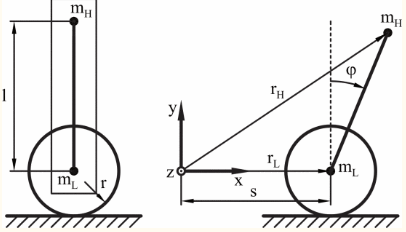
\includegraphics{images/dynamics}
\caption{Point mass model of self balancing bot}
\label{fig:dynamics}
\end{figure}

\clearpage

The assumptions are as follows (refer to figure \ref{fig:dynamics}) :
\begin{enumerate}
  \item The non-uniformly distributed mass within the body has been reduced to point masses to make analysis easy.
  \item mh and ml are connected to each other having distance l between them.
  \item The rotational inertia Jw is also taken in account.
\end{enumerate}

\section{Modelling of self-balancing platform}

The self-balancing platform is an ordinary platform with a servo attached indirectly to it through a beam. The servo is controlled by another micro-controller and this micro-controller receives feedback from a gyroscope placed on the platfrom which tells the micro-controller the displacement of the platform from its mean position. The platform here is again approximated as a point mass being displaced from its mean position.

\section{Working}

\begin{figure}[H]
\centering
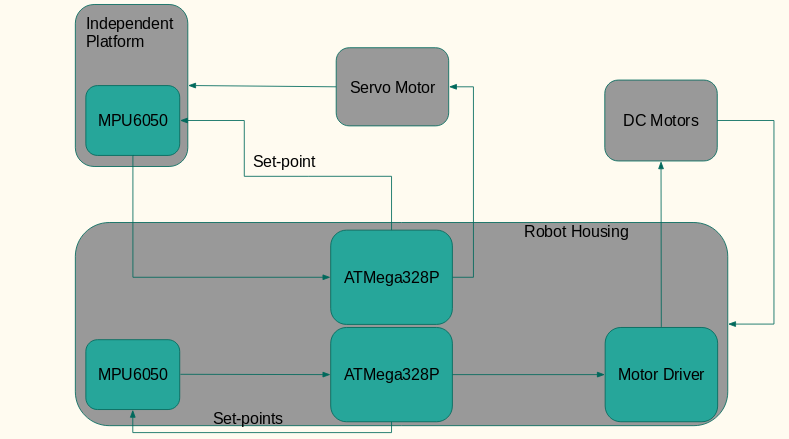
\includegraphics[width=\textwidth,height=\textheight,keepaspectratio]{images/control}
\caption{Control flow of the entire system}
\label{fig:control}
\end{figure}

Figure \ref{fig:control} shows the overall control flow of the whole system. The system works by correcting the errors in the position of the bot or platform with respect to their respective set point. \newline
If the bot is pitched forward (forward tilting motion), its new position as calculated by the gyroscope is dfferent from the set point initialized in the arduino. Hence the bot accelerates in the same direction of the tilt to compensate for the change in the the mean position. As the system is not an ideal system, the acceleration in the previous case might cause the bot to tilt in the other direction now. And hence the bot will now accelerate in a direction opposite to that before to achieve a stable state. \newline
The PID values in the control algorithm are altered on a trial and error basis to minimize these oscillations and to arrive at the stable mean position quicker.\\

The self balancing platfrom also works in a very similar manner. The main difference is that instead of giving the platfrom a linear acceleration to compensate for displacement from set point, the platfrom is simply rotated in the direction opposite to displacement using a servo. \newline
During the motion of the bot, the platfrom very rarely gets displaced from its mean position by a large enough margin to be corrected by a gyroscope. The platform is barely even displaced because :
\begin{enumerate}
  \item The structure is very rigid for there to be noticeable changes with small angular displacement.
  \item The bot accelerates with a very less acceleration value as it aims to stabilize about a point and a high acceleration would lead to the bot going out of control. This less value of acceleration is not enough to displace the platfrom from its mean position.
\end{enumerate}
